\chapter{Experiments}

\section{Pickle Research Campus}\label{prcdata}

We collected a sample dataset between June 22nd and August 10th, 2012 at the
University of Texas's J.J.\ Pickle Research Campus.  To survey the campus, the
system was placed in a golf cart and driven on most work days on irregular
routes. Total observation time amounted to twenty hours in 48 observation runs
containing a total of more than 37,000 individual two-second observations.

\begin{figure}
  \centering
  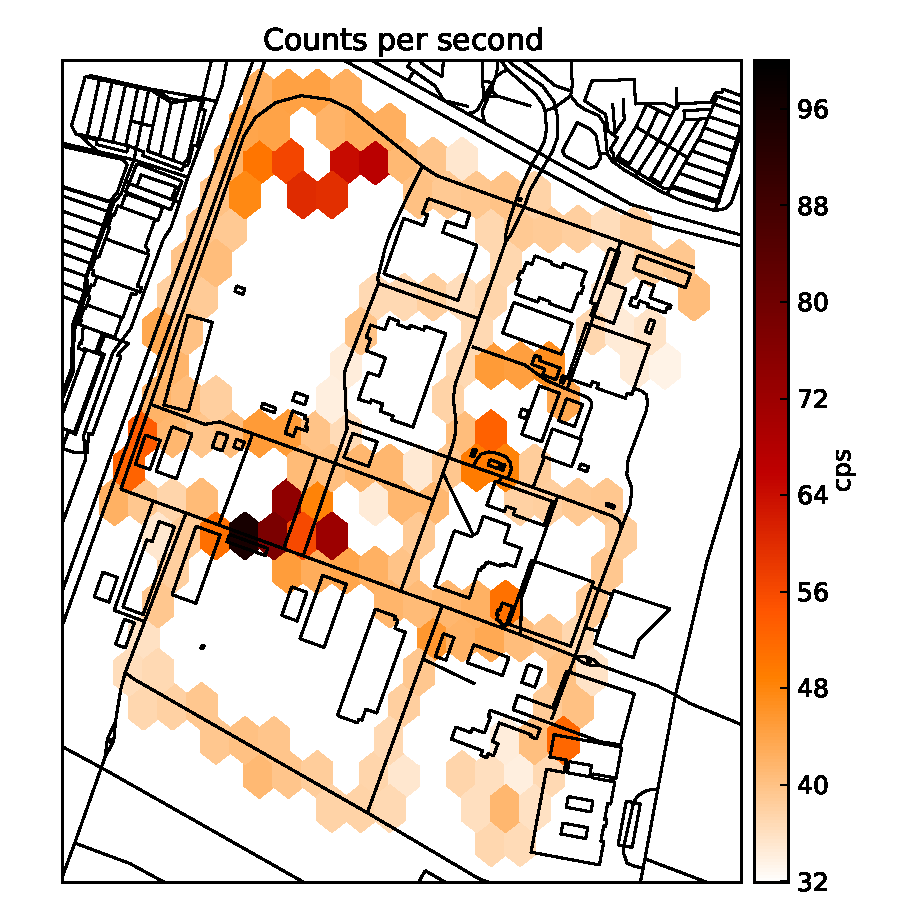
\includegraphics[width=4in]{figures/prc-cps.pdf}
  \caption{A map of J. J. Pickle Research Campus with gamma counts per second
    overlaid.  The campus is approximately 0.33 sq.\ mi., with north
    corresponding to up.  Areas of elevated background include the radioactive
    materials storage facility at the northwest corner and a cluster of large
    brick buildings near central campus.}
  \label{prc-cps}
\end{figure}

The natural gamma background varies spatially and temporally due to many natural
factors.  Our surveys revealed a spatially varying natural background across
Pickle Research Campus. A map of average radiation levels over several weeks is
shown in Fig.\ \ref{prc-cps}. Background activities vary spatially by a factor
of two due to natural and artificial sources.

\subsection{Poisson distribution assumption}

Our algorithmic approach relies on the underlying Poisson distribution of
radiation data.  To test the validity of this assumption, Poisson dispersion
tests were performed on the dataset as a function of spatial scales. The Poisson
dispersion test determines whether a given set of observations could plausibly
have been drawn from the same Poisson distribution \cite{Rao:1956vp}. The test
computes a dispersion parameter \(D\), defined by:
\begin{equation}
D = \frac{\sum_{i=1}^N (x_i - \bar{x})}{\bar{x}},
\end{equation}
where \(\bar{x}\) is the mean of all observations \(x_i\) and \(N\) the total
number of observations. This parameter is \(\chi^2\)-distributed with \((N -
1)\) degrees of freedom. A \(p\) value can be computed for \(D\), indicating the
probability that the observed distribution of values would arise from a
Poisson-distributed random variable. For example, dividing our dataset into
125-meter grid cells, we find that on average, \(p = 0.33\); this falls to \(p =
0.17\) for 250-meter cells, indicating that counts are not perfectly
Poisson-distributed.

To quantify this, the index of dispersion was computed for all grid cells at
various cell sizes. The index of dispersion \(V\) is a measure of the variance
of a distribution, compared to its mean:
\begin{equation}
V = \frac{\sigma^2}{\mu},
\end{equation}
where \(\mu\) is the distribution's mean and \(\sigma^2\) its variance. The
variance of a Poisson distribution equals its mean, so the index of dispersion
is expected to be one. Fig.\ \ref{poisson-dispersion} shows mean indices of
dispersion for various grid cell sizes, demonstrating that smaller cells tend to
have count rate distributions closer to the expected Poisson distribution, as
expected. To account for this, we adjusted the dispersion parameter \(V\) in
Eq.~\ref{vars} to match the mean index of dispersion for grid cells at a
chosen spatial scale.

\begin{figure}
  \centering
  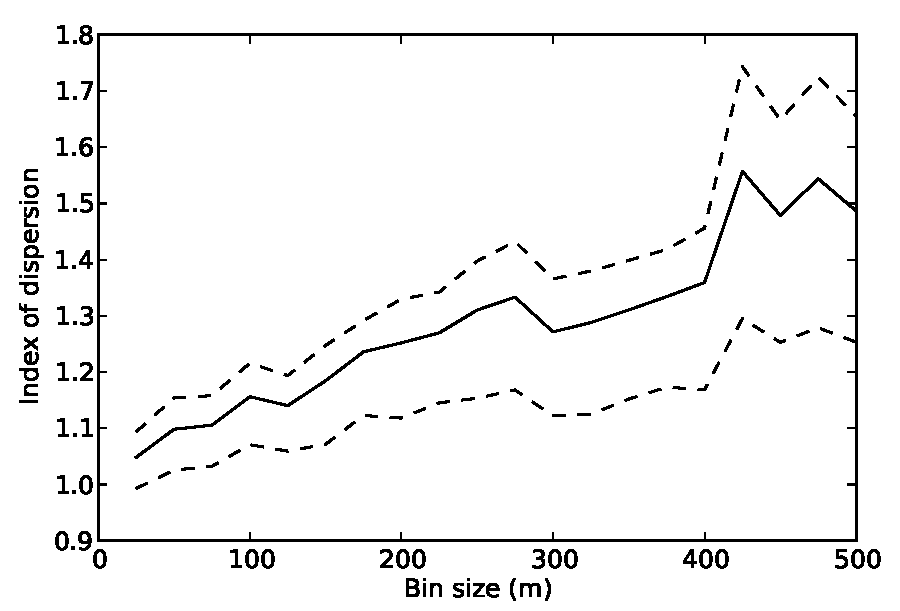
\includegraphics[width=4in]{figures/poisson-dispersion.pdf}
  \caption{Mean, minimum and maximum index of dispersion of counts in each
    energy bin for all grid cells, at specified grid sizes. An index of 1 is
    consistent with a Poisson distribution.  As expected, smaller cells more
    closely match the Poisson distribution, while larger cells have additional
    variance.}
  \label{poisson-dispersion}
\end{figure}

\subsection{Comparing spatial and temporal variation}

Our dataset at the Pickle Research Campus revealed not only spatial but temporal
variation in background. To compare the temporal variation to the spatial
variation, the observation area was divided into grid cells 250 meters on each
side, and each day's set of observations was compared to two or more previous
days using the SCRAM algorithm. Fig.\ \ref{scr-distribution} shows the
distribution of \(D^2\) recorded over several dozen passes through the area. For
comparison, it also plots the \(D^2\) values calculated by comparing each grid
cell's spectrum to a fixed reference cell, rather than comparing it to the same
cell on a previous day.

\begin{figure}
  \centering
  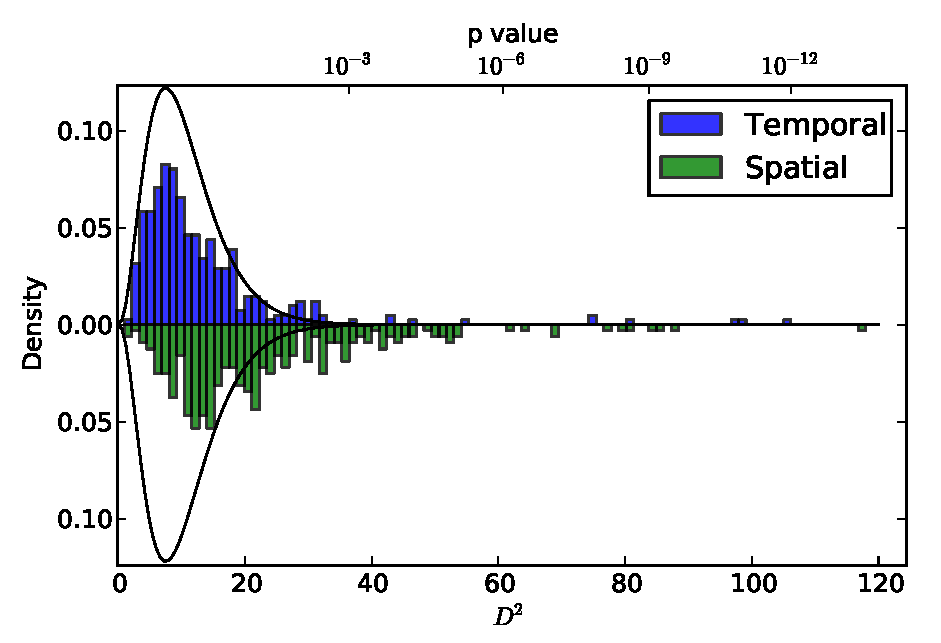
\includegraphics[width=\textwidth]{figures/scr-distributions.pdf}
  \caption{Distribution of the SCR anomaly statistic \(D^2\) in 250-meter grid
    cells in the sample dataset, with a \(\chi^2\) distribution (\(\text{df} =
    7\)) overlaid. The upper histogram is the result of comparing each grid cell
    to the same cell on the previous day; the lower histogram compares each cell
    to a fixed reference cell, showing spatial rather than temporal
    variation. The lower distribution is clearly shifted to the right.}
  \label{scr-distribution}
\end{figure}

The spatial distribution is clearly shifted to the right, indicating that there
is more spatial variance than temporal variance. This validates the assumption
of the SCRAM algorithm that it is best to compare spectral observations to
previous observations made in the same place, rather than observations made at
other locations. In other words, background spectra vary much more spatially
than they do temporally. This suggests that alarm thresholds may be set lower
when using the SCRAM method to perform anomaly mapping, giving higher
sensitivity without increased false alarm rates.

The presence of \(p < 10^{-3}\) anomalies in Fig.~\ref{scr-distribution} is not
unusual. The \(p\)-values are computed under the \(\chi^2\) distribution, which
the data do not follow perfectly. There are, of course, some true variations in
natural background in the data. Also, some spectral comparisons were made with
little data -- because we drove irregular routes, a spatial bin may only contain
a few seconds of data, giving an extremely poor estimate of the spectrum in that
bin.

\section{Blind testing at football games}\label{football}

To validate the detection algorithm it was necessary to perform blind
tests. We needed a large area in which radioactive sources would likely appear
and could be found using the SCRAM technique. University football games meet
these criteria: with 100,000 fans in attendance, it is statistically likely that
at least one or two fans will have recently been exposed to a medical
radioisotope.

First, we took background spectral measurements of the stadium. Measurements
were collected on three separate mornings while the stadium was empty. The
scintillator was carried in a backpack up and down every set of stairs in the
stadium, with a team of three or four walkers operating in shifts.

As seen in Fig.~\ref{stadium-heatmap}, the stadium has a varying natural
background. In particular, the west upper deck appears to have a higher
background activity than the rest of the stadium. The stadium was initially
built with only the lower inner stands, and the west upper deck was constructed
later, with the north and east decks following later. Consequently, different
batches of materials went into the concrete making up the decks, and the
different materials may have different levels of thorium, uranium, and
potassium, the primary contributors to concrete's natural background radiation.

\begin{figure}
  \centering
  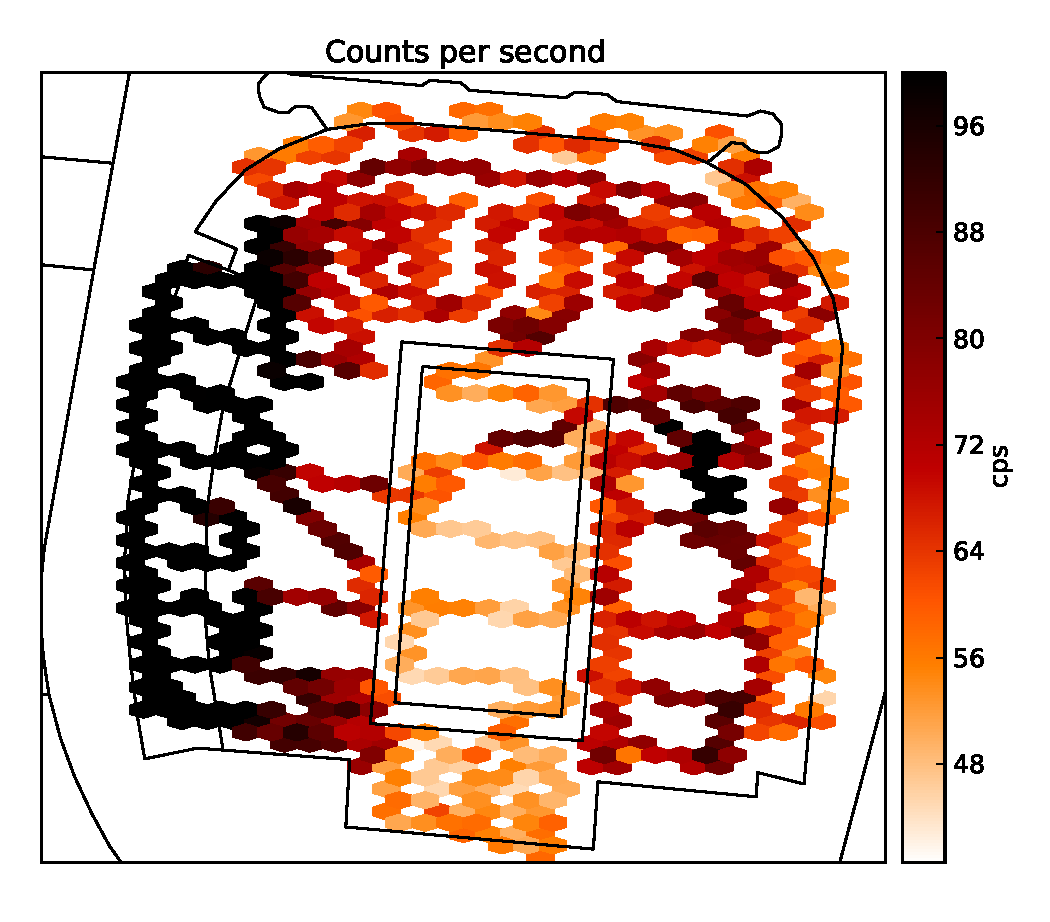
\includegraphics[width=\textwidth]{figures/stadium-heatmap.pdf}
  \caption{An October 1, 2012 background measurement of the stadium. The more
    active area on the left is the west upper deck, which appears to have a
    relatively high natural background radiation. (North is up.) Radiation
    levels are typically \(\approx 10 \,\mu\)R/hr in the west deck, or roughly
    one fiftieth of the dose rate experienced in an airplane traveling at 40,000
    feet.}
  \label{stadium-heatmap}
\end{figure}

This effect can be seen in Fig.~\ref{stadium-concrete}, where spectra from the
east and west decks of the stadium are compared. There are no spectral peaks
unique to the west upper deck; instead, the potassium-40 peak and the low-energy
Compton-scattered region are shifted up, indicating higher levels of
potassium-40 and other natural radioisotopes within the concrete. Levels of
potassium and thorium are known to vary by an order of magnitude within
different samples of concrete, so this is unsurprising.\cite{Ryan:2011wh}

\begin{figure}
  \centering
  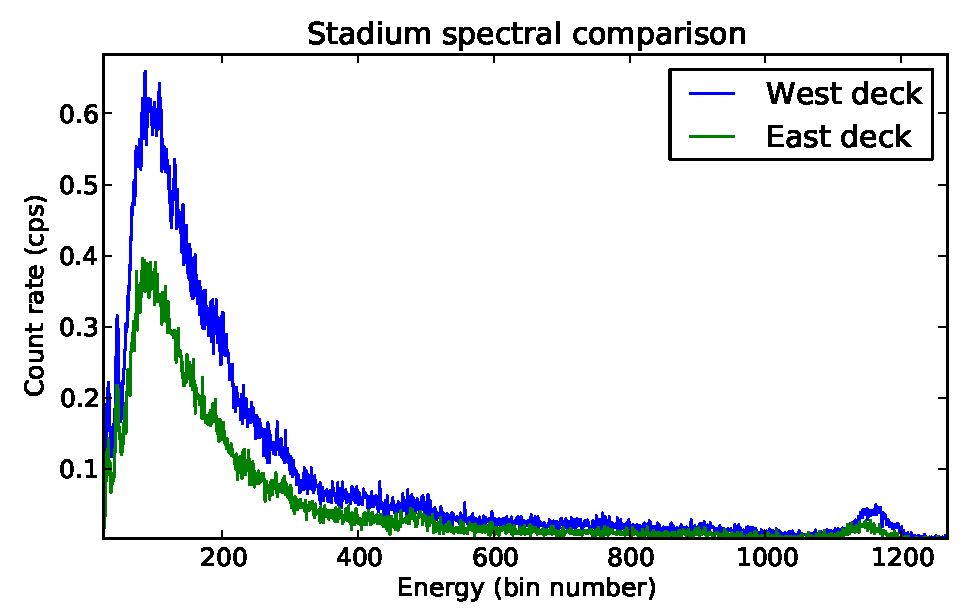
\includegraphics[width=\textwidth]{figures/stadium-concrete.pdf}
  \caption{The west upper deck of the football stadium shows higher source
    activity than the rest of the stadium. Here, the upper spectra is the west
    upper deck, while the lower spectra is the east deck; both spectra are
    normalized to show count rates in counts per second. The west deck evidently
    has more potassium-40 (the peak on the right) and more Compton-scattered
    low-energy gamma activity.}
  \label{stadium-concrete}
\end{figure}

During one background collection run, a calibration problem occurred while
collecting data on the west upper deck. When examining spectra afterwards, it
appeared that the potassium-40 peak had vanished. It appears now this was due to
a shift in calibration while collecting the data; the peak was consequently
``smeared'' across a wide range of energy bins, making it vanish. We did not
remove this data, and so anomaly detection on the west upper deck will tend to
exaggerate spectral changes until sufficient background is collected to hide the
problem. Future work will need to provide automatic energy calibration in
real-time, so spectra are not smeared. It may be possible to calibrate
retrospectively by using known background peaks in the data.

Next, spectra were collected at three football games, each with attendance of
roughly 100,000. While collecting spectra we wore Polimaster personal radiation
detectors, which use a small scintillator to monitor dose rates and provide
alarms when rates suddenly increase. We used these detectors to localize
sources.

We experienced several difficulties collecting data. During our first game, on
October 6, 2012, we were able to detect an iodine-131 source; however, frequent
GPS errors and cabling problems prevented us from recording a complete map of
the stadium. With no real-time way of monitoring the data collection system in
the backpack, we had no way of telling when cables had come unplugged, and we
lost valuable time. We only recorded roughly a quarter of the lower decks, along
with the north and east upper decks.

By the second game on October 20, we had developed a monitoring system that
could be accessed over WiFi from a smartphone. We reinforced cable connections
and were able to record a complete map of the stadium. Two anomalies were
detected, shown in Fig.~\ref{oct20-stadium-scr}. GPS drift was a problem:
despite indicating a good signal lock, the GPS location tended to drift in
random directions when parts of the sky were obscured by overhead
obstacles. Cleaning up this data will be essential for future analysis.

\begin{figure}
  \centering
  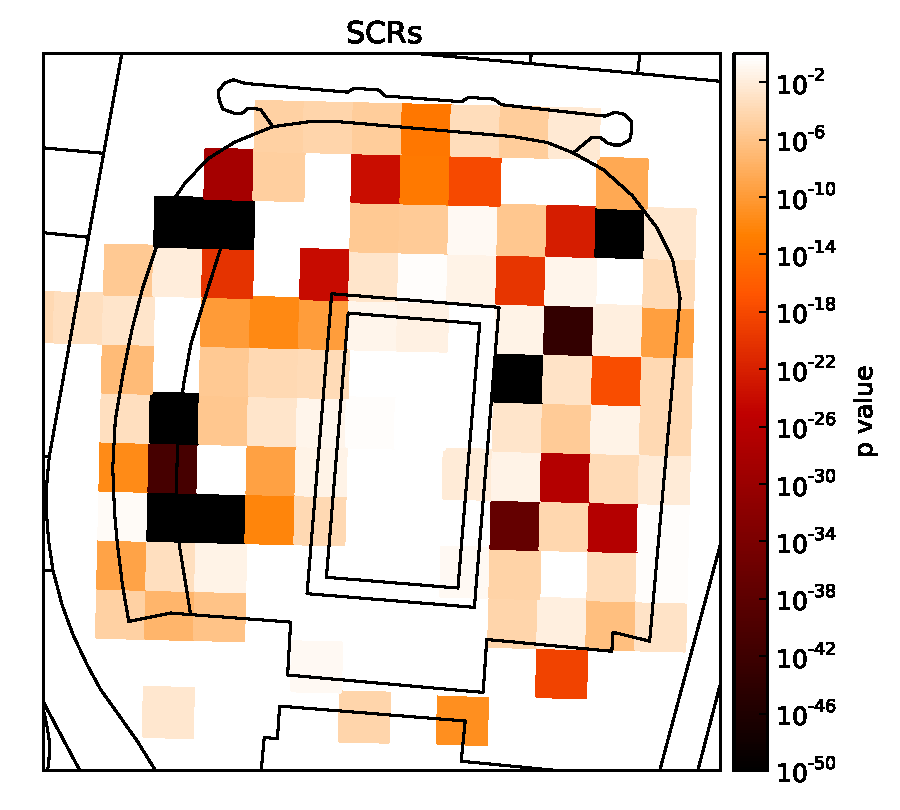
\includegraphics[width=\textwidth]{figures/oct20-stadium-scr.pdf}
  \caption{An SCR map of the stadium on the October 20th run. At the top left
    and lower left, confirmed spectral anomalies are shown. At mid-right is an
    anomaly caused by GPS drift: while investigating the top left anomaly, GPS
    position drifted across the field due to a large overhang blocking the GPS
    signal, and so an anomaly was recorded on the east side of the stadium.}
  \label{oct20-stadium-scr}
\end{figure}

Upon examining the spectra, both spectral anomalies were determined to be
technetium-99m. A representative spectrum is shown in
Fig.~\ref{oct20-spectrum}. One anomaly was easily detectible with our personal
radiation detectors, which alarmed as we walked past; this anomaly was
investigated with a portable identifying spectrometer and confirmed as
technetium-99m. Another was not noticed during the game but appeared in anomaly
maps generated afterward, as the source was smaller or farther away from our
chosen route.

\begin{figure}
  \centering
  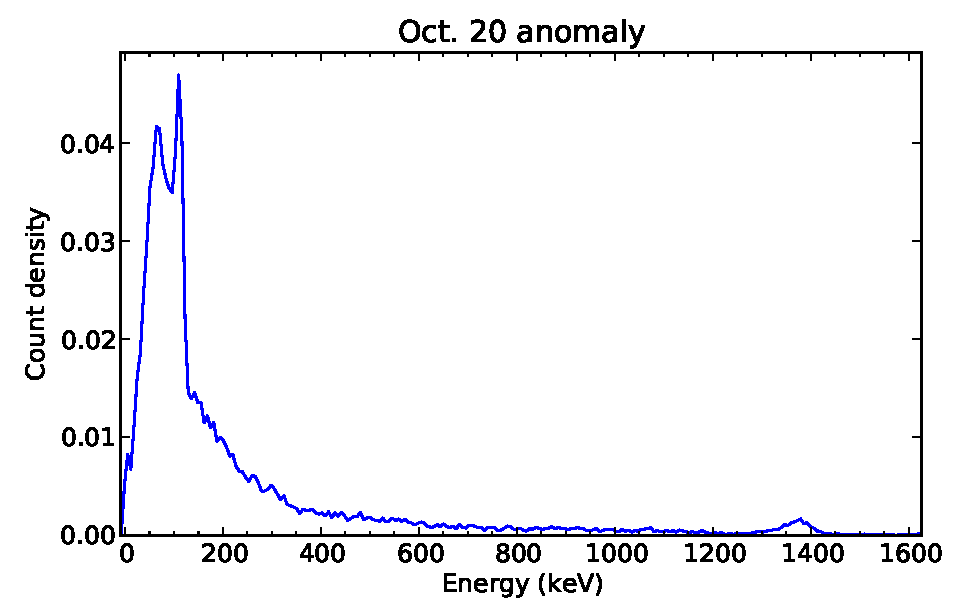
\includegraphics[width=\textwidth]{figures/oct20-spectrum.pdf}
  \caption{A smoothed spectrum recorded during the October 20th data collection
    run at the football stadium. The spectrum is normalized so that its integral
    is one. This appears to be technetium-99m from a medical patient inside the
    stadium. Environmental Health and Safety verified this with a portable
    identifying spectrometer.}
  \label{oct20-spectrum}
\end{figure}

Another game was recorded on November 10, with complete coverage of the stadium
again achieved. Two Tc-99m anomalies were again observed, one with an activity
100 times greater than background at a distance of less than a meter.

These tests demonstrated the utility of the SCRAM system for the monitoring of
public events and large areas. The system was able to accurately identify
spectral anomalies caused by medical radioisotopes, allowing further
investigation by Environmental Health and Safety or the University of Texas
Police Department. Some false positive results were produced, and the causes of
these will need to be investigated. One potential cause of false positives is
the comparison of spectra from consecutive games: if a medical source is present
during one game but missing during the next, this may be counted as an
anomaly. A principled system to exclude anomalous data from background
measurements will be required.

\section{Minimum detectable sources}

To test the performance of the SCRAM algorithm, we performed a simulation to
calculate the minimum detectable radioactive source size at a variety of
distances. We selected a straight stretch of road on the northwest corner of the
Pickle Research Campus and simulated the injection of a cesium-137 source at
various distances from the road into the collected background data.

To choose our alarm threshold, we used the anomaly statistics distribution data
shown in Fig.~\ref{scr-distribution}, selecting a threshold which gives a 1\%
false-alarm rate in our example dataset. For temporal comparisons of spectra,
this threshold is \(D_A^2 = 83\), while for purely spatial comparisons the
result is \(D_A^2 = 113\). We computed the minimum detectable source sizes for
both thresholds, and the results are given in Fig.~\ref{minimum-detectable}.

\begin{figure}
  \centering
  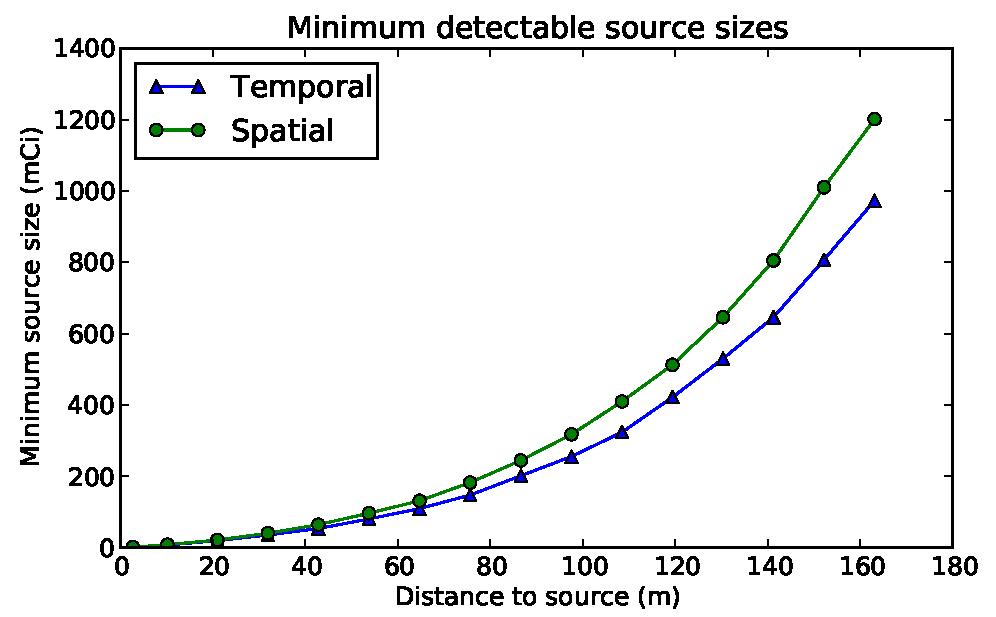
\includegraphics[width=\textwidth]{figures/minimum-detectable.pdf}
  \caption{The minimum detectable cesium-137 source sizes at various distances
    away from the detector's path, using both temporal and spatial comparisons
    of spectra. Total observation time was 136 seconds.}
  \label{minimum-detectable}
\end{figure}

These results show that taking advantage of the exact prior background spectrum
at each location leads to better detection performance by approximately 20\%. Of
course, smaller sources would be detectable with a much larger scintillator or
with a much longer observation time. It will also be necessary to validate these
results experimentally.

\section{Bus route simulation}

To evaluate the feasibility of using the SCRAM algorithm with public transit
vehicles to monitor a wide area, we performed a simulation using Capital Metro
bus routes in downtown Austin, Texas. The results demonstrated the feasibility
of the SCRAM method for real-time monitoring of a wide area, such as the
downtown of a city.

Bus routes were extracted from shapefiles made available by Capital
Metro.\cite{capmetro} We selected only those routes which passed through
downtown Austin multiple times daily, excluding infrequent express routes; the
resulting routes are shown in Fig.~\ref{downtown-map}, along with a map of
Austin.

\begin{figure}
  \centering
  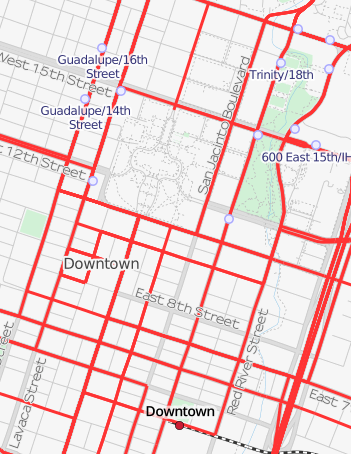
\includegraphics[width=0.5\textwidth]{figures/downtown-transport-map.png}
  \caption{A map of downtown Austin bus routes. Data provided by
    OpenStreetMap,\cite{osm} with rendered map by Andy Allan.}
  \label{downtown-map}
\end{figure}

To simulate observations made by passing buses, a simulated bus traversed each
route defined in the shapefiles. The shapefiles define a route as a series of
connected points; we simulated a bus which stopped at each point for ten
seconds. Given the typical spacing between points of 115 meters, this comes out
to roughly 25 miles per hour average speed for each bus. Each bus was modeled as
traveling its route exactly once. Additional simulation runs could be performed
to have buses make multiple passes.

Background radiation for the area of downtown Austin was simulated. A
representative background spectrum was selected from the Pickle Research Campus
data and simulated at a constant activity of 50 counts per second (plus random
Poisson variation) across the observation region; a 1 Ci point source with a
spectrum taken from Pickle Research Campus was simulated downtown; and a 30 Ci
source with a spectrum taken from a brick building at Pickle Research Campus was
placed at the Texas State Capitol, simulating the higher activity from its
granite construction.

For background observations, twelve separate passes were simulated with the
aforementioned background sources. A 3.5 Ci cesium-137 source was then injected
at the site of the Texas State Capitol at a point which is 240 meters from the
nearest bus routes. At this distance, the source contributes roughly 10 counts
per second to the normal background rate of 50 cps. Using a simple personal
radiation detector which looks for an anomaly in total count rates several
standard deviations above background, this anomaly would not be detected.

Twelve bus passes were made with the injected source, producing an anomaly map
shown in Fig.~\ref{downtown-scrs}.

\begin{figure}
  \centering
  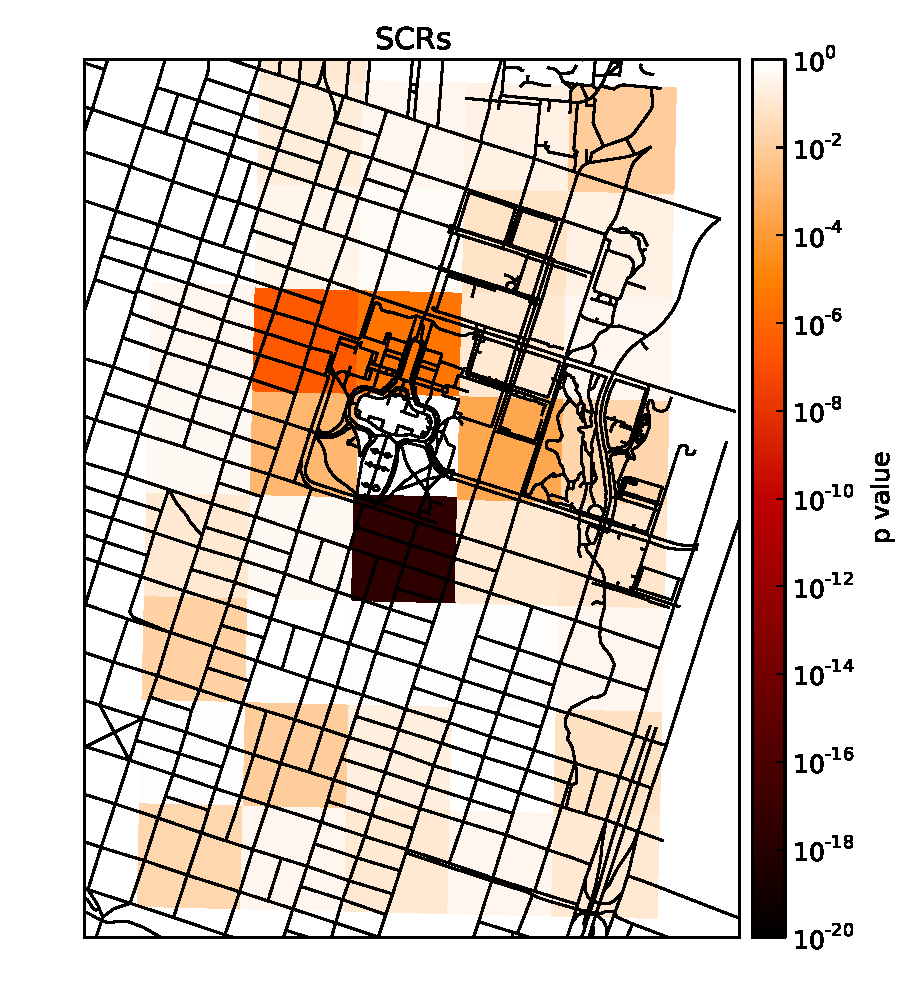
\includegraphics[width=0.8\textwidth]{figures/downtown-injected-scrs.pdf}
  \caption{A 3.5 Ci cesium-137 source has been injected at the site of the Texas
    State Capitol in this image. The nearest bus routes are shown in
    Fig.~\ref{downtown-map}, and are at least 240 meters away from the
    source. The anomaly was detected nevertheless.}
  \label{downtown-scrs}
\end{figure}

This simulation demonstrates the feasibility of the SCRAM system for wide-area
surveillance using public vehicles. Because buses pass through downtown Austin
frequently, many observations can be collected and small anomalies detected
relatively quickly.

In the future we hope to collect accurate wide-area data of downtown Austin or
another area to enable better simulations. Also, the simulation system does not
account for attenuation caused by the presence of large buildings in Austin;
more detailed simulation and experimental work would be needed to determine
detection capabilities when sources are shielded by buildings, vehicles, or
crowds.
